\chapter{FPGA Implementation}
\label{Chapter-FPGA-Implementation}

\section{Tools Used}
% Todo: Review Vivado edition
This work's CNN inference accelerator was implemented and optimized for FPGA platforms using the Xilinx Vivado Design Suite - HL System Edition 2019.2 \cite{Vivado-Design-Suite}. Vivado Design Suite is a software suite developed by Xilinx for its FPGA devices for analysis and synthesis of Hardware Description Language (HDL) designs, written in VHDL or Verilog. It is superseding Xilinx ISE \cite{Xilinx-ISE}, as a complete rewrite, with additional features for System-on-Chip (SoC) design and High-Level Synthesis (HLS). The tools used in this work are Xilinx Vivado HLS, Xilinx Vivado IDE, and Xilinx SDK.

\subsection{Vivado IDE}
Xilinx Vivado Integrated Design Environment (IDE), released in 2012, is the basis for all Xilinx tools. It serves as a GUI front-end for the Vivado Design Suite. All Vivado Design Suite tools integrate a native TCL interface, which can be accessed from IDE's GUI and the TCL console. Vivado IDE can compile, synthesize, implement, place and route FPGA hardware designs written in high-level languages such as C/C++, and HDLs such as VHDL and Verilog.

In addition, using the IP Integrator tool, hardware systems can be designed by graphically connecting IP blocks and configuring them through their GUI, with no coding involved, hence, accelerating the design process. Integration automation features such as auto-connecting and auto-configuring blocks further accelerate the design process. IP blocks can be created using the integrated IP Packaging functionality for VHDL or Verilog designs and via the Xilinx HLS tool for C/C++ designs. Xilinx also provides many IP blocks for free, including but not limited to on and off-chip-network IPs, memory blocks and memory management IPs, I/O interface IPs, and even various compute IPs. There are also additional IP's that can be purchased from Xilinx or even other vendors and developers.

After the design process is completed, a bitstream can be created and then downloaded to the target FPGA device to run as a standalone hardware device or in combination with firmware running on the FPGA's integrated ARM cores. The device's firmware is developed, compiled, and deployed using the Xilinx Software Development Kit (SDK) tool.

Designs can be tested on IP level or ever system-wide using the IDE's integrated simulator or any other RTL simulator. Moreover, Vivado IDE provides various debug tools that, combined with Integrated Logic Analyzer (ILA) IPs, can scan, check, and visualize the system's behavior during runtime.

\subsection{Vivado High-Level Synthesis (HLS)}
Xilinx Vivado High-Level Synthesis (HLS) \cite{Vivado-Design-Suite-User-Guide-High-Level-Synthesis}, currently rebranded as Xilinx Vitis HLS, is a tool included in the Xilinx Vivado Design Suite, allowing for a higher level of abstraction design of HDL systems. Vivado HLS synthesizes C/C++, SystemC and OpenCL functions into IP blocks, generating their VHDL and Verilog HDL designs that can then be implemented into hardware systems using Vivado and its Block Design tool.

While HLS accepts non-hardware-optimized code, it provides a set of directives that can instruct the synthesis procedure to implement a specific behavior, optimization, and resource management. Directives are optional and do not affect the input code's behavior. Their usage can both benefit the generated IP's performance and even hurt it when not used correctly. Furthermore, constraints, like clock period, clock uncertainty, and FPGA target, are added to the HLS synthesized IP blocks to ensure the desired behavior and performance.

A C/C++ testbench is used to debug the input code's behavior prior to synthesis, which should feed the input code with test data and check its output for correctness. Verification of the exported IP block is done using the C/RTL Cosimulation functionality, which uses the same C/C++ testbench, but replaces the function's call with the exported IP block call.

\subsubsection{Synthesis Report}
A synthesis report is created whenever HLS successfully synthesizes an IP Block, showing various performance and resource utilization metrics. Using the synthesis report, the designer can easily find and target the bottleneck to further optimize their design in terms of both performance and resources. Since Vitis HLS 2020.1, the report summary also contains the aforementioned information per loop per module, making the optimization procedure even more targeted. Some of the metrics are presented and explained below.

\begin{itemize}
	\item \textbf{Latency:} The number of clock cycles required for a complete run of a module or loop.
	\item \textbf{Iteration Latency:} The number of clock cycles required for running a single iteration of a module or loop.
	\item \textbf{Iteration/Initiation Interval (II):} The number of clock cycles required before a module can accept new input or a loop can initiate a new iteration.
	\item \textbf{Pipelined:} Whether a module or loop is implemented using a pipelined architecture.
	\item \textbf{Area:} The number of hardware resources a module requires for its implementation into the target FPGA. The hardware resource types are Block RAM (BRAM) and Ultra RAM (URAM), Digital Signal Processing (DSP) units, Flip Flops (FF), and Lookup Tables (LUT). A table is also given on the detailed report, showing the number of hardware resources required for every hardware component type, which include DSPs, Expressions, First-In-First-Out (FIFO) queues, Instances, Memories, Multiplexers, and Registers.
\end{itemize}

\subsubsection{Optimization Directives}
As mentioned above, HLS provides a set of directives for design optimization in terms of latency, throughput, and resource utilization of the exported IP block. Those directives can be added directly into the input code in the form of pragmas that the preprocessor can read. Another way of adding directives is by creating a new solution and automatically adding them to it. Every solution combines a set of directives and configurations into TCL files, one TCL file per solution. Multiple solutions can be created, each with different directive combinations and configurations. This way allows for better experimentation and fine-tuning of the design. Some optimization directives are presented and explained below.

\begin{itemize}
	\item \textbf{Interface:} The top-level function's arguments have to be mapped to RTL ports to configure the IP block's functionality. The interface directive specifies each argument's port type.
	\item \textbf{Stream:} By default, the top-level function's array arguments are implemented as RAM channels. However, when data are being produced or consumed sequentially, a more efficient data type is to use FIFOs, which can be specified using the stream directive.
	\item \textbf{Pipeline:} Given an \emph{Initiation Interval (II)} parameter, the pipeline directive reduces the number of clock cycles a function or loop can accept new inputs, targeting \emph{II} clock cycles, by allowing the overlapped execution of operations.
	\item \textbf{Unroll:} Given a \emph{factor}, the unroll directive unrolls a loop \emph{factor} times, creating multiple instances of the loop body, that can then be scheduled independently or run in parallel.
	\item \textbf{Loop Flatten:} Allows perfectly nested loops, loops that no logic is injected between them, to get collapsed into a single loop, reducing latency. Essentially, it handles all the indexing logic of the loop flattening.
	\item \textbf{Loop Merge:} Merges consecutive loops, often initialization loops, reducing overall latency and resource utilization.
	\item \textbf{Resource:} Specifies the resource for a variable to get implemented.
	\item \textbf{Array Partition:} By default, every array is implemented as a set of at least one BRAM unit with a single read and a single write port. The array partition directive partitions an array into multiple smaller arrays or assigns each array's element to its register. This partitioning increases the read and write ports of the array on the hardware level, allowing for parallel I/O and computations. In the potential expense of more memory instances and more register, array partitioning can improve overall throughput and performance of memory bounded applications.
	\item \textbf{Array Map:} The array map directive combines multiple small arrays into a single large one, to avoid BRAM waste on small arrays, which can occupy a BRAN unit for just a few elements.
	\item \textbf{Array Reshape:} Reshapes an array of many elements of small bit-width to an array of fewer elements but of higher bit-width, increasing the sequential BRAM access speeds.
	\item \textbf{Data Pack:} Similar to the array reshape directive, the data pack directive combines struct data fields to a single scalar of higher bit-width.
	\item \textbf{Dataflow:} Enables parallel execution of functions and loops, increasing throughput and latency.
	\item \textbf{Inline:} Similar to C/C++ macro preprocessor functionality, the inline directive injects a function's body to each of its calls, reducing latency and initiation interval due to lower function call overhead.
	\item \textbf{Allocation:} Limits the number of hardware resources used for implementing the IP block, and may result in hardware sharing and latency increase.
	\item \textbf{Latency:} Limits the minimum and maximum latency in clock cycles.
\end{itemize}

\subsection{Xilinx SDK and Xilinx Vitis IDE}
Xilinx Software Development Kit (SDK) \cite{Xilinx-SDK}, currently unified with SDSoC and SDAccel into Vitis Unified Software Platform, is an IDE for embedded-software development Xilinx's microprocessors. Based on the Eclipse IDE \cite{Eclipse-IDE}, it includes a C/C++ editor, a compilation toolchain for ARM microprocessors with automatic Makefile generation, system performance analysis and optimization tools, and several debug and profiling tools. It is used to create applications that run on the ARM cores either external to the FPGA die or internal like on the MPSoCs. Often those applications play the role of the coordinator/master that organizes, schedules, and configures the FPGA hardware. They often handle the external I/O, like data transfers to and from storage devices (SD cards, Hard Drives, Flash Memories, etc.) or Ethernet, to and from volatile memory (RAM, BRAM, etc.). They can also handle the data pre-processing needed to feed the FPGA hardware. Furthermore, multi-core processors can be utilized simultaneously using bare-metal applications. If multi-processing is required with a sophisticated scheduler, Linux applications can be built and run on Linux operating systems like PetaLinux \cite{PetaLinux} and FreeRTOS \cite{FreeRTOS}.

Xilinx SDK is strongly coupled with the Xilinx Design Suite and its hardware designs and bitstreams. After the successful implementation and bitstream generation of the hardware design from Vivado IDE, Xilinx SDK imports the project's hardware wrapper to generate the Board Support Package (BSP) and various C/C++ libraries useful for communication with and configuration of the FPGA hardware.

Xilinx SDK can create three main types of applications; bare-metal, First Stage Boot Loader (FSBL), and Linux applications. Their main difference is on the way the application is loaded onto the system's processor.
\begin{itemize}
	\item \textbf{Baremetal:} A bare-metal application is loaded using the SDK's built-in functionality that can program the FPGA (PL part) and load it onto the corresponding ARM core through the JTAG port.
	\item \textbf{FSBL:} A FSBL application is a set of files generated by the SDK that, when put on the root folder of the system's primary storage device, e.g., SD card, are read during the system's boot-up, triggering a boot loader sequence. The system has to be appropriately configured, typically configuring some jumpers and switches on development boards to instruct the processor to read the FSBL files. When the bootloader sequence is triggered, programming of the FPGA and loading the application are done using the primary storage device as a source, with no need for an external computer, and Xilinx SDK or JTAG.
	\item \textbf{Linux:} A Linux application is similar to the FSBL one, with the only difference that a Linux operating system is required to be running on the system's processor. Similarly, the Linux OS is loaded using the primary storage device. When Linux is fully loaded, the application can be started like any other Linux application through the provided console window to program the FPGA and run it.
\end{itemize}
A console window is used for input and output functionality using the UART port in all application types.

Debugging applications is as simple as regular locally running applications using the built-in System Debugger or other debugging tools like GDB \cite{GDB}. In addition, Vivado IDE's Hardware Manager can be used in combination with SDK's System Debugger to debug hardware designs and their driver applications. Vivado IDE's Hardware Manager connects to the hardware's ILA IPs, enabling the monitoring in real-time of the hardware's state concerning the driver application's state.

\section{FPGA Platforms}
\label{sec:FPGA-Platforms}
This work focuses on the two FPGA platforms available in the lab, the Xilinx ZCU102 Evaluation Kit, and the FORTH QFDB. Conveniently, both platforms integrate the same Zynq UltraScale+ MPSoC XCZU9EG-2FFVB1156E.

\subsection{Xilinx Zynq UltraScale+ MPSoC XCZU9EG-2FFVB1156E}
The Xilinx Zynq UltraScale+ Multi-Processor System-on-Chip (MPSoC) \cite{DS891-Zynq-UltraScale-MPSoC-DataSheet-Overview} family of products integrates multiple ARM Cortex-A53 and Cortex-R5 cores processing system (PS) and a Xilinx UltraScale programmable logic (PL) architecture in a single chip with on-chip memory, multiport external memory interfaces and several peripheral connectivity interfaces.

Some key features of XCZU9EG-2FFVB1156E are:
\begin{itemize}
	\item Quad-core 64bit ARM v8-A Cortex-A53 with L1/L2 cache.
	\item Dual-core 32bit ARM v7-R Cortex-R5 with L1 cache.
	\item ARM Mali-400 MP2 graphic processing unit.
	\item 256KB on-chip ECC memory.
	\item Xilinx 16nm FinFet+ programmable logic fabric.
	\item 600k system logic cells.
	\item 548k CLB Flip-Flops.
	\item 274k CLB LUTs.
	\item 32.1Mb Block RAM.
	\item 2520 DSPs.
\end{itemize}

\subsection{Xilinx ZCU102 Evaluation Kit}
The Xilinx ZCU102 Evaluation Kit \cite{ZCU102-User-Guide} \cite{ZCU102-Product-Overview} (Figure \ref{fig:ZCU102-board-overview}) is a general-purpose development board for rapid prototyping based on the aforementioned UltraScale+ MPSoC. It provides a complete platform with an SD card as a primary storage device, 4GB 64bit ECC DDR4 SODIMM RAM, 512MB DDR4 component memory for PL, and a power delivery system. It also provides various configuration switches and jumpers, and all major peripherals and interfaces such as PCIe Gen 2x4 slot, SATA, Ethernet, HDMI input and output, DisplayPort, USB, JTAG, and UART.

\begin{figure} [H]
	\centering
	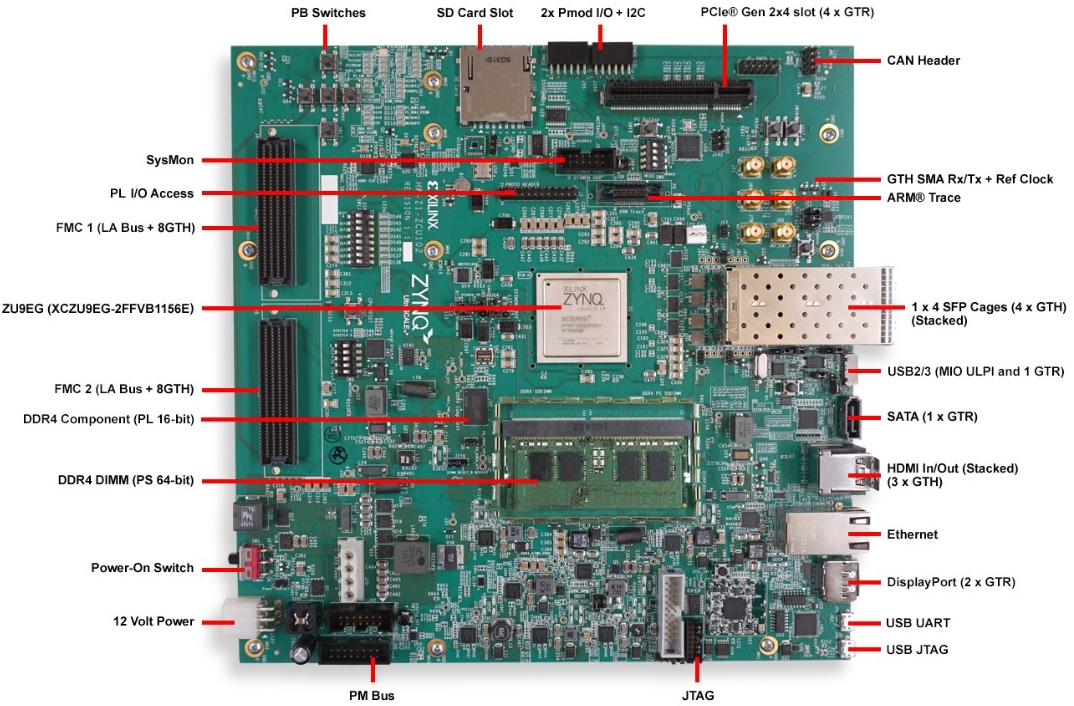
\includegraphics[width=\textwidth]{Images/Hardware/ZCU102-board-overview.jpg}
	\decoRule
	\caption[Xilinx ZCU102 Evaluation Board overview]{Xilinx ZCU102 Evaluation Board overview: \href{https://www.xilinx.com/products/boards-and-kits/ek-u1-zcu102-g.html}{URL}}
	\label{fig:ZCU102-board-overview}
\end{figure}

\subsection{FORTH QFDB}
The Quad-FPGA Daughter Board (QFDB) (Figure \ref{fig:forth-qfdb-daughterboard}) \cite{Implementation-and-Impact-of-an-Ultra-Compact-Multi-FPGA-Board-for-Large-System-Prototyping}, developed by the Foundation of Research and Technology Hellas (FORTH) \cite{FORTH}, combines four of the aforementioned MPSoCs, interconnected with each other. It is a complete platform as well, which provides 16GB of DDR4 memory and an M.2 Solid State Drive (SSD), and some peripherals and interfaces such as Ethernet, JTAG, and UART.

It is designed to be used in servers, with other QFDBs running in parallel, creating a network of FPGAs. The QFDB enables massive hardware designs to be split and deployed into multiple FPGA devices or even multiple QFDB boards. It also enables the deployment of hardware designs into a high number of FPGAs for increased parallelism.

\section{The Platform}
For this work, a platform was created capable of CNN inference on FPGA devices. This platform had to be created with flexibility and versatility in mind to be able to be transferred to other FPGA devices while being based on the Xilinx ZCU102, which was available in the lab. It should also be scalable to enable multi-FPGA implementations, and it should be extendable to enable for easy adding of new layer types and new layer accelerators. Furthermore, it should be able to run various CNN models' inference, but most importantly, it should provide easy experimentation and development of hardware accelerator architectures.

The basic building blocks of this platform consists of its volatile and non-volatile memory, and its compute engine. Figure \ref{fig:platform-block-diagram} depicts the platform's block diagram, whose functionality is explained below. It should be noted that everything described below is implemented on the aforementioned Xilinx ZCU102 Evaluation Kit.

\begin{figure} [H]
	\centering
	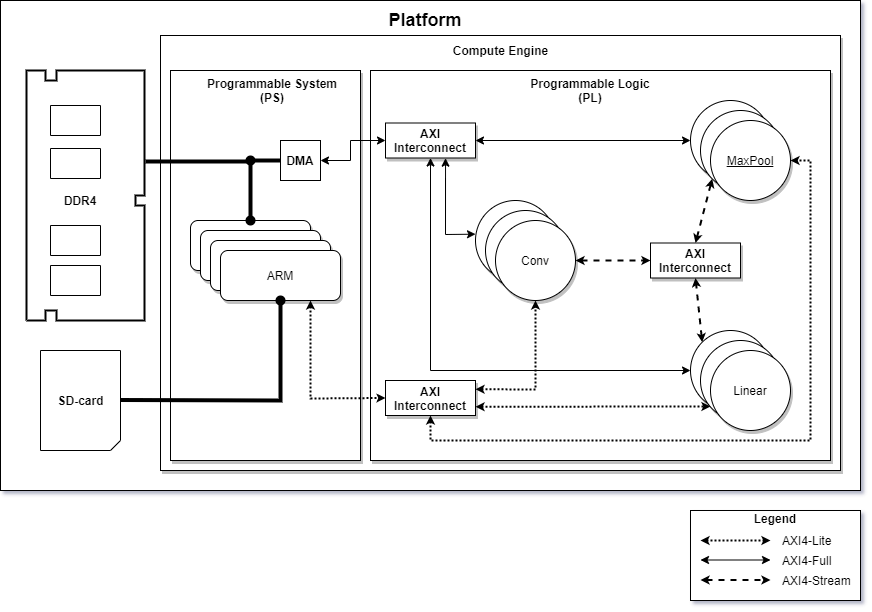
\includegraphics[width=\textwidth]{Images/Platform/platform.png}
	\decoRule
	\caption[The platform's block diagram]{The platform's block diagram.}
	\label{fig:platform-block-diagram}
\end{figure}

\subsection{Non-Volatile Memory}
This platform's non-volatile memory serves as a storage medium for all the data that networks require for their inference, which include the initialization data (network model configurations, parameters (weights and biases), class labels), and the input data (e.g., images). An SD-card is used as the non-volatile memory for this platform (also depicted as an SD-card in Figure \ref{fig:platform-block-diagram}). However, with some software extensions, other storage devices can also be used, such as SATA hard drives or even M.2 SSDs (on other FPGA platforms, e.g., QFDB). Moreover, external storage devices can also be utilized, via the Ethernet port through local-network/Internet, or via the JTAG port to avoid copying files over and over again on the platform's primary storage device but also to enable the single-source access for multiple FPGA devices.

While SD-cards have little bandwidth than other storage devices like SATA drives and M.2 SSDs, the non-volatile memory's purpose is to initialize the platform, which is a one time cost, and feed it with input data. When the platform is on its initialization phase, the initialization data from its non-volatile memory are transferred to its volatile memory to get later used from the compute engine. Because most, if not all, networks' initialization data fit in the volatile memory, leaving a lot of empty memory space, input data are also transferred, filling as much space as possible to utilize the volatile memory's high bandwidth for input data consumption. Consequently, the SD-card's low bandwidth can be safely ignored.

If the input data are large enough to not completely fit in the volatile memory and their consumption is faster than their feed through the SD-card, a faster storage device should be used. However, in this work's experiments, this has never been the case.

\subsection{Volatile Memory}
The platform's volatile memory consists of two types of memory devices, the DDR4 modules found on the ZCU102 and the on-chip BRAM. The ZCU102 also provides a separate DDR4 component accessible from the FPGA's PL part, however for simplicity and generality (it is not provided on all FPGA platforms) purposes, and because it provides lower bandwidth compared to the DDR4 modules, it is not utilized on this platform.

The platform's primary memory medium is the DDR4 memory modules  (also depicted as a DDR4 module in Figure \ref{fig:platform-block-diagram}) connected to both the PS and PL parts of the device. As mentioned before, it stores and serves all the required data for the platform to run. Those data are read from various files found on the non-volatile memory, in this case, the SD-card, using the ARM cores found on the PS part, and are then stored onto the DDR.

The DDR has to feed the PL part with data in chunks because, as explained in section \ref{sec:Memory-Footprint}, the integrated BRAM cannot store the whole network's parameters and activations. Consequently, every network's layer has to know where to find and how to access every piece of data it requires, information that is found on the platform's software structures and passed to the layers using the ARM cores during the setup phase.

On this platform, there is no central BRAM component that every accelerator accesses. Instead, every accelerator should implement its own BRAM, without permitting access to others. It should be the only one to know how to manage its storage. Of course, to fulfill the accelerator's needs in bandwidth, read and write ports, and latency, it can implement its BRAM as it requires, and utilize individual registers.

\subsection{Compute Engine}
The compute engine consists of both the PS and PL part of the FPGA device, which includes the ARM cores and the FPGA accelerators, respectively. While the bulk of the computation is handled by the PL part, the PS part handles the more sophisticated computations, such as the input data pre-processing and the accelerator configuration and scheduling.

In this platform, a network can be run only if its layers are supported by either software or hardware implementations. Software implementations are running on the ARM cores, and hardware implementations are the FPGA accelerators. By allowing both types of implementations, this platform expands its flexibility. This can not only help the development stage of FPGA accelerators by comparing their outputs with the ones generated by the software implementation, but it can also help to fully utilize the device's resources by running parts of even whole layers on the ARM cores in parallel to the hardware accelerators. Furthermore, layers that have not yet been implemented in hardware can easily be implemented in software for experimentation purposes, such as the Depth Concat layer found on the GoogLeNet (Figure \ref{fig:GoogLeNet}).

As shown in Figure \ref{fig:platform-block-diagram}, in this work, three layer types have been implemented in hardware; the Convolutional (Conv) layer, the Max-Pooling (MaxPool) layer and the Fully-Connected (Linear) layer. In addition, multiple instances of the same layer type can also be added in the platform to enable for either parallel execution of different inferences with different inputs or even different network models, or better pipelining in a single inference. This is discussed in detail in section \ref{sec:CNN-Scheduling}.

In this work, every accelerator implements a layer type, and, therefore, the platform assumes that every accelerator can handle and compute a whole layer type's computation. Every accelerator comes with its driver, which is integrated into the platform's software. The driver is responsible for setting up its accelerator, which includes setting the layer's hyperparameters and passing the information of where to find its parameters (weights and biases), its input data, and where to send its output data. Also, the driver handles the accelerator's interrupts, which,  in this work, only includes the accelerator completion interrupt.

The assumption that every accelerator implements a whole layer type simplifies the accelerator's driver. As a result, the driver does not have to know its accelerator's inner workings and architecture, except for its aforementioned settings, treating it as a black box with inputs and outputs. However, those settings are the same for every implementation of the same layer type; hence, experimenting with different architectures is made easy without developing a different driver for every single architecture. The driver can be reused on the same layer type accelerators, letting the engineer focus their efforts on the accelerator's architecture. Of course, every different layer type needs different settings; therefore, different drivers.

It is worth mentioning that every accelerator has an AXI4-Lite \cite{UG1037-Vivado-Design-Suite-AXI-Reference-Guide} slave port through which it can get configured. All accelerators' AXI4-Lite slave ports are connected to a Xilinx AXI SmartConnect IP \cite{PG247-SmartConnect-Product-Guide}, onto its master ports. The AXI SmartConnect, a replacement of the AXI Interconnect IP, acts as a router, providing a single slave port that is finally connected to the Zynq's (ARM cores) master port. AXI SmartConnect automatically detects the port's protocol, in this case, AXI4-Lite, and adjusts its ports accordingly. This creates a hardware connection so that the software can access and configure the platform's accelerators. Details on the AXI protocol are given in section \ref{sec:AMBA-AXI4-Interface-Protocol}.

\subsection{I/O}
\label{sec:IO}
As explained in previous sections, the I/O bandwidth provided to any hardware platform plays an essential role in its performance due to the CNNs' high bandwidth requirements. Hence, the platform should implement a network for its accelerators to enable the communication between them, the PS part, the DDR, and each other. There are three ways for high bandwidth communication, which are discussed below.
\begin{itemize}
	\item \textbf{Memory-Mapped I/O (MMIO):} In this method, the PS communicates with its PL part's accelerators using a global address space for both its main memory (DDR) and the accelerators' I/O extensions, mapping every memory component, such as the DDR, BRAM, and registers, onto its own address range. While it is straightforward to implement, it can create a bottleneck on random memory accesses onto the DDR, with each request costing up to 50 clock cycles for the DDR's initialization. Fortunately, this is not the case with burst accesses, which request only once a range of addresses so that there is only one initialization cost for a big transfer of data.
	\item \textbf{Streaming (AXI4-Stream):} Using streaming interfaces, such as the AXI4-Stream, continuous communication can be established between components in a FIFO manner. Every streaming connection creates a channel between the two components with a predefined FIFO size, with a producer-consumer behavior. Communication between hardware accelerators and the DDR can be established using the Xilinx AXI DMA IP \cite{PG021-AXI-DMA-Product-Guide}, which hides the DDR's initialization costs. However, AXI DMA requires knowledge of the data flow, and its function is instructed by the PS part for every transfer, increasing the system's complexity.
	\item \textbf{BRAM:} This method is an MMIO variation, which uses BRAM IPs to store the required data on-chip, taking advantage of the BRAM's high bandwidth. Data are transferred from the DDR to the BRAM in bursts using a Xilinx CDMA IP \cite{PG034-AXI-Central-Direct-Memory-Access-Product-Guide} connected to a Xilinx BRAM Controller IP \cite{PG078-AXI-BRAM-Controller-Product-Guide} and its Xilinx Block Memory Generator IP \cite{PG058-Block-Memory-Generator-Product-Guide}. Though, a major constraint is that the data have to be small enough to fit into the chip's BRAM, which is in the order of a few MBs in size.
\end{itemize}

As explained in section \ref{sec:Memory-Footprint}, the integrated BRAM cannot store the parameters for most layers. There is the case that parameters can be transferred in chunks to the central Block Memory IP; however, this creates further complexity and bandwidth bottleneck due to the low number of read and write ports. Therefore, the BRAM method described above cannot be used in this platform.

Hence, the question that arises is which method is more suitable for this platform, the MMIO or the Streaming one. To answer it, a test system was created, integrating a simple IP, created using Vivado HLS, that adds a specific value to its input data, and then returns its output data. The input data are generated on the PS part and are stored on the system's DDR. The IP's output is returned to the PS part and stored on its DDR. Then the PS validates the outputs to ensure their correctness. The IP's input and output ports are implemented both as streams and as MMIO.

The test measures the average number of clock cycles it takes for both implementations to process 40MB of data in chunks of 40kB. The chunk's size was selected greedily, because most, if not all, accelerators' requests need to be at least 40kB. The time measurement includes the input data transfer from the DDR to the IP's BRAM, the input data processing, and the output data transfer from the IP's BRAM to the system's DDR. Both implementations were tested with 32 and 128 input and output ports bit-width. The test's results are shown on table \ref{tab:MMIO-vs-Stream}.

\begin{table}[H]
	\caption[MMIO vs Stream]{MMIO vs Stream: Processing 40MB data of 40KB bursts, showing a slight advantage over the MMIO method.}
	\label{tab:MMIO-vs-Stream}
	\centering
	\begin{tabular}{lll}
		\toprule
		\textbf{Port bit-width} & \textbf{MMIO avg. cycles} & \textbf{Streaming avg. cycles}\\
		\midrule
			32-bit 	& 62700922 & 65611580\\
			128-bit & 15761270 & 16201797\\
		\bottomrule\\
	\end{tabular}
\end{table}

Both implementations for both port bit-widths show similar results, with a slight advantage over the MMIO implementation. Selecting MMIO for the primary method of data feeding the accelerators benefits the platform not only in terms of bandwidth, according to the slight advantage depicted on table \ref{tab:MMIO-vs-Stream}, but also in terms of simplicity of both software and hardware implementation and efficiency of hardware resources.

Consequently, the connection between the accelerators and the PS part and its DDR is established using the MMIO method, as shown on the platform's block diagram (Figure \ref{fig:platform-block-diagram}). Every accelerator has an AXI4-Full \cite{UG1037-Vivado-Design-Suite-AXI-Reference-Guide} master port, which is connected to a Xilinx AXI SmartConnect IP, onto its slave ports. The SmartConnect's master port then gets connected onto the Zynq's slave port. Communication to the DDR is established via the Zynq's slave port, and an integrated DMA found on the PS part.

However, the streaming method cannot be dismissed entirely, as it is perfect for communication between accelerators. Passing a layer's activations to its next layer, in terms of hardware means passing the accelerator's output data to the next accelerator as input data. Implementing this data transfer in a streaming manner avoids transferring data from the FPGA to the DDR and then transferring them back to the FPGA using the MMIO method, which can be a significant bottleneck. As a result, every accelerator can optionally have additional input stream and output stream ports. The accelerators driver configures it to either use the MMIO or the streaming method.

It is vital that every accelerator implements at least the MMIO method, to avoid running into deadlocks. For example, let there be a system with one instance of a layer type's accelerator, and the accelerator's output stream needs to get connected back to the same accelerator's input stream. A deadlock occurs when the output stream is full while the accelerator has not finished its execution. In this case, the accelerator hangs, waiting for the stream to accept more data, while the stream hangs, waiting for its data to get consumed. This problem can easily be tackled by simply sending the accelerator's outputs to the DDR using the MMIO method, and when its execution is complete, it can then read them back again from the DDR.

A Xilinx AXI4-Stream Switch IP \cite{PG085-AXI4-Stream-Infrastructure-IP-Suite-Product-Guide} is used to create a star topology \cite{Network-Topology-Wikipedia} stream network, connecting every accelerator's stream ports, as shown on the platform's block diagram (Figure \ref{fig:platform-block-diagram}). Every connection is assigned an address in the AXI4-Stream Switch IP before synthesis so that the TDEST signal of the AXI4-Stream protocol can be set accordingly by the sender accelerator. The AXI4-Stream Switch IP was preferred to the AXI4-Stream Interconnect IP because the latter is the same as the Switch, but it also allows connections of streams with different characteristics in the cost of some hardware resources. However, all accelerators are implemented with the same stream characteristics, so the Interconnect's use is redundant.

\subsection{AMBA AXI4 Interface Protocol}
\label{sec:AMBA-AXI4-Interface-Protocol}
The AMBA AXI4 (Advanced eXtensible Interface 4) \cite{UG1037-Vivado-Design-Suite-AXI-Reference-Guide} is the AMBA interface specification from ARM, which is integrated into the Xilinx Design Suite tools to offer a single standard interface and simplify the IP integration. All Xilinx IPs that require any configuration or large amounts of data implement at least one of the AXI4's variation. The AXI4 protocol has three variations for different use cases.
\begin{itemize}
	\item \textbf{AXI4-Full:} Used for high-performance memory-mapped applications, supporting bursts of up to 256 beats.
	\item \textbf{AXI4-Lite:} The simplest of all three variations, with the least hardware resources requirements. It is used for low-throughput memory-mapped applications, usually for accessing control registers, with every transaction having a burst length of one
	\item \textbf{AXI4-Stream:} Used for high-speed streaming unidirectional data transfers from master to slave, supporting multiple data streams using the same set of shared wires, and multiple data widths withing the same interconnect.
\end{itemize}

This platform makes usage of all three variations for different purposes, as shown on its block diagram (Figure \ref{fig:platform-block-diagram}). The AXI4-Lite is used for configuring the accelerators; the AXI4-Full is used to implement the accelerators' MMIO, as described in section \ref{sec:IO}, and the AXI4-Stream is used to create the star topology network between the accelerators.

\subsection{Software}
The platform's software was developed using the Xilinx Vitis IDE, previously known as Xilinx SDK. Xilinx Vitis provides the necessary compilation toolchain, and the ability to program the FPGA and run software on the ARM cores. This platform cannot function without its software. It should be clarified that everything that is considered a software part runs on the device's processor (ARM cores). The software consists of the accelerators' drivers, the scheduler, the application logic, and the user interface.

The drivers are responsible for the communication between the software and hardware of this platform. They are used to handle the initialization, configuration, and use of each hardware component. They also handle the accelerators' various interrupt events, affecting the software's execution. Every accelerator's driver has to implement several functions with specific functionality and naming scheme, creating an abstraction layer between the drivers and the rest of the software. This makes integrating a new accelerator into the platform easier because the other software parts "know" how to use the new driver, expanding the platform's modularity. Moreover, it is essential that the interrupt service routines are kept as small as possible to avoid missing any other interrupt events while executing them.

The application logic is responsible for configuring the platform depending on the user's input. It handles the parsing of the network model configuration files, the loading of the network's initialization data (parameters and labels), the input data preprocessing, and the accelerator execution according to the scheduler's instructions. It is designed with data arbitration in mind, in order to easily experiment with different data types used in the network's parameters and activations. The application logic's data type is the same with the one used in the accelerators' architecture, and when set, it propagates to the whole software.

For the sake of simplicity, a command-line interface implements the user interface. Most FPGA platforms have a UART port that can be used to print messages, accept user input, and debugging. Therefore, this platform utilizes the UART port for its user input requirements. From the application's menus, the user can select several functions, among which there is a self-test routine that tests the platform's integrity, a network model selection with its corresponding parameters, an image count selection, and an option to run both software and hardware implementations of every layer for output data checking. While not implemented, the user interface can be expanded to a graphical user interface using a standalone program or server, running on a host PC that reads and writes the aforementioned UART port.

The scheduler is the last but not least, part of the platform's software. It is responsible for scheduling all the necessary tasks for the network's inference to execute. A task can be executing a layer or a group of layers either in software or using the hardware accelerators. The scheduler is also responsible for scheduling the input and output methods of each accelerator (MMIO and Streaming), the input source and output destination. Per platform implementation, there might be needed a different scheduler strategy. For example, there is a different strategy for a platform with only one instance per accelerator type, and a different one when there are multiple, or when the accelerators' execution can be pipelined. For more information on the platform's scheduler strategies see section \ref{sec:Scheduler-Strategies}

A simplified flowchart of the platform's software execution can be seen in figure \ref{fig:platform-flowchart}. On system boot-up, the drivers are discovering and initializing all peripheral devices, such as the SD-card and the UART ports. Afterward, they discover and initialize every accelerator existing in the FPGA's PL part. During this step, the interrupt handlers are also getting set. Next, the user interface asks the user for which network from the available it should run its inference and all the aforementioned running options. Given the user's input, the application logic reads the network model file, parses it, and loads it to the platform's memory. It also loads the network's parameters, labels, and input data. Then, for each input data, the scheduler adds the tasks into a list to be run whenever possible. Then, for every task, the corresponding accelerator is set up and triggered to run using its drivers. The platform finishes when there are no more tasks to be run and input data to get processed.

\begin{figure} [H]
	\centering
	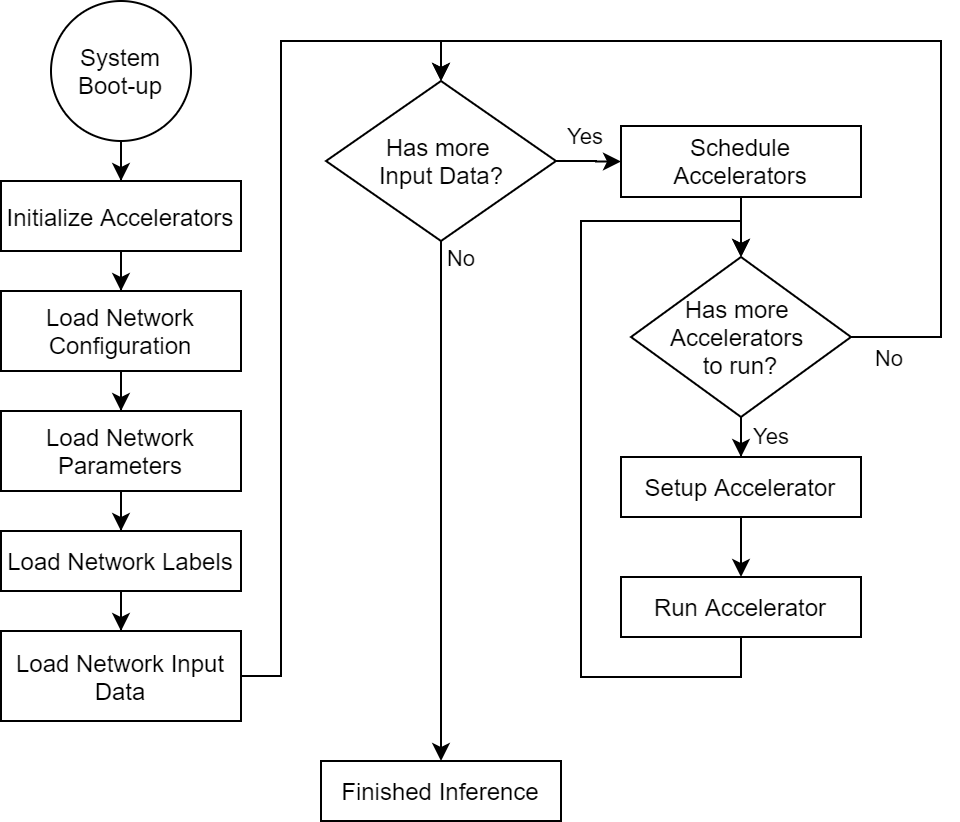
\includegraphics[width=\textwidth]{Images/Platform/PlatformFlowchart.png}
	\decoRule
	\caption[The platform's flowchart]{The platform's flowchart.}
	\label{fig:platform-flowchart}
\end{figure}

\subsection{Scheduler Strategies}
\label{sec:Scheduler-Strategies}
Scheduling can play a significant role in the platform's performance. As mentioned in the previous section, the scheduling strategy is dependent on the platform's implementation and goals. The number of same-type accelerator instances and whether the platform is throughput or latency optimized, all affect the strategy selection. To study and demonstrate the various strategies, a MATLAB model of a CNN network's inference execution was created that can compute the execution characteristics of any CNN network model. This work's main CNN network is AlexNet, on which all experiments below are based.

The MATLAB model creates a timed schedule of a CNN inference depending on its hyperparameters. It computes the number of clock cycles a layer requires for its full execution, and depending on the strategy selected, it places the layer's execution start and finish timestamps. The clock cycles required for every full execution is equal to the sum of the clock cycles needed per assembly instruction to be executed. The number of clock cycles required for every assembly instruction can be set on the MATLAB model's parameters. However, for simplicity, all instructions are considered to run in a single clock cycle.

The following figures show the starting clock cycle, the ending clock cycle, and the duration of every layer, wherever there are colored boxes. Every colored box has its label, defining the layer that it represents. The label is coded as the layer's type and its serial number; Conv for convolutional layers, MaxPool for max-pooling layers, and Linear for fully-connected layers. It should be noted that the ReLU activation function is embedded into the convolutional and fully-connected layers, as shown on algorithms \ref{alg:Convolution-Layer-with-ReLU} and \ref{alg:Fully-Connected-Layer-with-ReLU}.

\subsubsection{Serial Strategy}
A baseline schedule was created using a serial execution strategy, as shown in figure \ref{fig:serial-execution}. In this strategy, every layer starts when the previous layer has finished generating all its outputs. This strategy can be used when there is only one accelerator instance per layer type, and the accelerators do not support layer pipelining. It is also an excellent strategy for debugging and validating the platform and its accelerators because of its simplicity.

\begin{figure} [H]
	\centering
	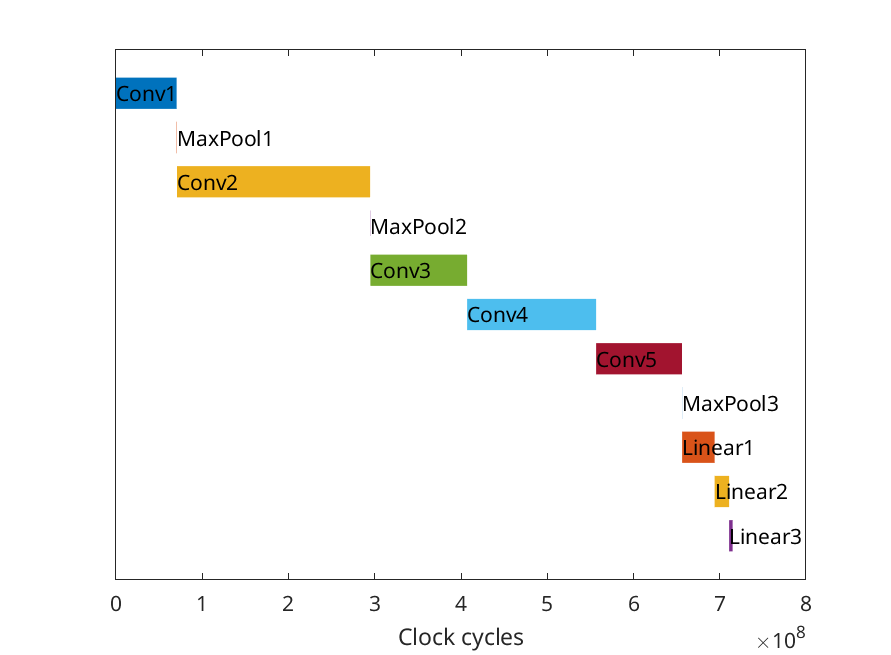
\includegraphics[width=\textwidth]{Images/Scheduling/Serial.png}
	\decoRule
	\caption[AlexNet serial execution]{AlexNet serial execution: Convolution layers consume 90\% of total clock cycles needed for a full inference.}
	\label{fig:serial-execution}
\end{figure}

It can be observed that using the serial execution strategy, around 90\% of the total clock cycles is consumed from the convolutional layers, and almost 0\% is consumed from the max-pooling layers. Hence, according to Amdahl's law, see section \ref{sec:Amdahls-Law}, the convolutional layers should get the most hardware resources for their accelerators to create as much parallelism as possible, while fully-connected layers come next, and max-pooling layers come last.

\subsubsection{Layer-Pipelining Strategy}
Another scheduling strategy is applying pipelining within the layers. In this strategy, a layer is fed with input data as soon as the previous layer generates a single output. This hides the next layer's latency as much as possible by computing outputs in parallel with the computation of its next-to-be-processed inputs. A schedule using the layer-pipelined strategy is shown in figure \ref{fig:layer-pipelined-execution}. To produce such a schedule using this strategy, it is considered to exist as many accelerators per layer type as needed. In this schedule, there are needed five instances of a convolutional accelerator,  three instances of a max-pooling accelerator, and three instances of a fully-connected accelerator.

\begin{figure} [H]
	\centering
	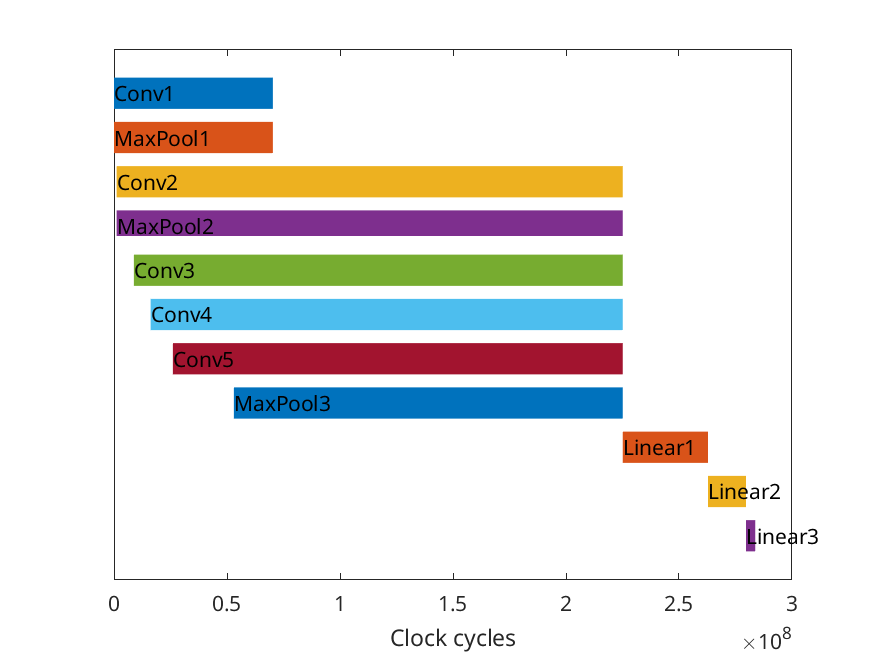
\includegraphics[width=\textwidth]{Images/Scheduling/Pipelined-1x.png}
	\decoRule
	\caption[AlexNet layer-pipelined execution]{AlexNet layer-pipelined execution: There is a speedup of almost 3 times compared to the serial strategy.}
	\label{fig:layer-pipelined-execution}
\end{figure}

The first four layers, Conv1, MaxPool1, Conv2, and MaxPool2 seem to start their execution immediately; however, this is not the case. In fact, they all start on different timestamps, each later from its previous one, but it just cannot be shown in figure \ref{fig:layer-pipelined-execution} due to the x-axis' scale. Conv1, MaxPool1, and Conv2 generate their first outputs in a few clock cycles compared to the x-axis scale. The same artifact appears on the finishing timestamps of the first two layers, Conv1 and MaxPool1, and the next six layers, Conv2 to MaxPool3.

From figure \ref{fig:layer-pipelined-execution}, it can be seen that the whole execution has significantly been reduced compared to the serial strategy shown in figure \ref{fig:serial-execution}, speeding it up almost three times.

However, to use the layer-pipelined strategy, the accelerators have to support it. This means that they need to process their inputs as soon as possible to generate their outputs. Because convolutional and max-pooling layers process their inputs in the 3D and 2D space, they have different implementation requirements to support layer-pipelining, compared to the fully-connected layers that compute their inputs in the 1D space.

Convolutional and max-pooling layers need to process their inputs in a way that they can generate outputs in a specific order. The optimal output order is the one that the next layer wants its inputs to be in, to also produce useful outputs for its next layer. The convolutional and the max-pooling layers produce outputs using cubes or squares of inputs, respectively, starting from the top left input of the grid. Those inputs are created from the previous layer, which also generated them using cubes or squares of inputs. Hence, the deeper the layer, the bigger the required cube or square of the first layer's inputs. Consequently, the optimal order of generating outputs starts from the top left and moving downwards and right in zones, always creating bigger and bigger cubes or squares. Figure \ref{fig:output-generation-order} depicts the order a convolutional or a max-pooling layer generates its outputs. It should be noted that the convolutional layers generate their outputs for all of their output channels, and then they move onto the next output.

\begin{figure} [H]
	\centering
	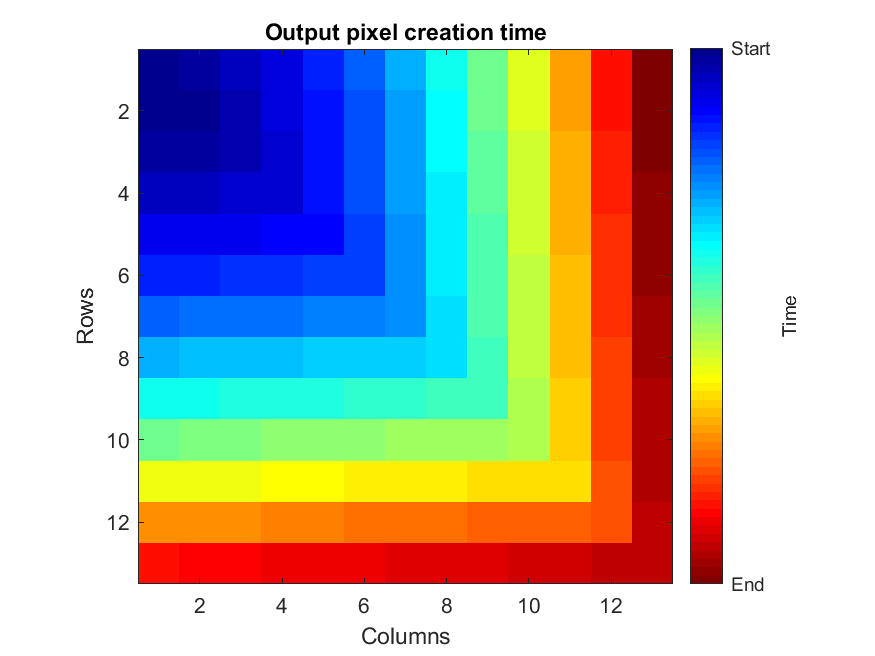
\includegraphics[width=\textwidth]{Images/Scheduling/Conv5-output-creation-time.png}
	\decoRule
	\caption[Convolutional and Max-Pooling layer output order for layer-pipelining]{Convolutional and Max-Pooling layer output order for layer-pipelining: Outputs colored in blue are generated before the red ones.}
	\label{fig:output-generation-order}
\end{figure}

In figure \ref{fig:output-generation-order}, every pixel is an output of a convolutional or max-pooling layer, and it is color-coded concerning the time it is generated, with blue and red colors representing the start and end, respectively, of the generation time.

However, layer-pipelining for convolutional and max-pooling layers significantly increased the implementation complexity of their accelerators. Also, caching weights and inputs in the accelerator's BRAM and registers can become a major obstacle due to their size and access patterns. Figure \ref{fig:Conv5-pixel-frequency} shows the input usage frequency for a convolutional or a max-pooling layer with a stride of one.

\begin{figure} [H]
	\centering
	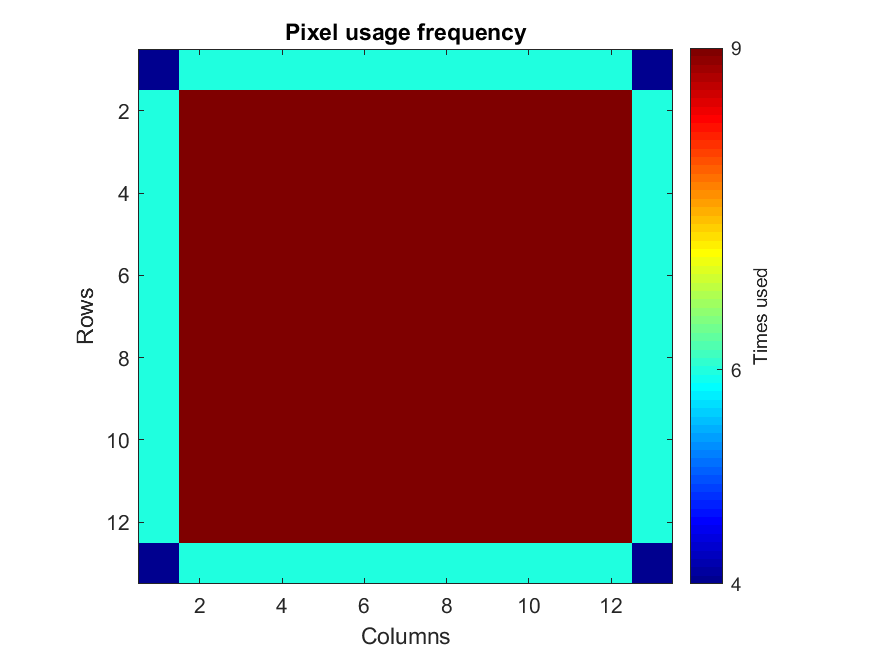
\includegraphics[width=\textwidth]{Images/Scheduling/Conv5-pixel-frequency.png}
	\decoRule
	\caption[Convolutional and Max-Pooling layer input pixel usage frequency using a stride of one]{Convolutional and Max-Pooling layer input pixel usage frequency a stride of one: Blue inputs are rarely used, while red ones are used frequently.}
	\label{fig:Conv5-pixel-frequency}
\end{figure}

Figure \ref{fig:Conv1-pixel-frequency} depicts the input usage frequency for a convolutional or max-pooling layer with a stride of four, showing even more complex access patterns.

\begin{figure} [H]
	\centering
	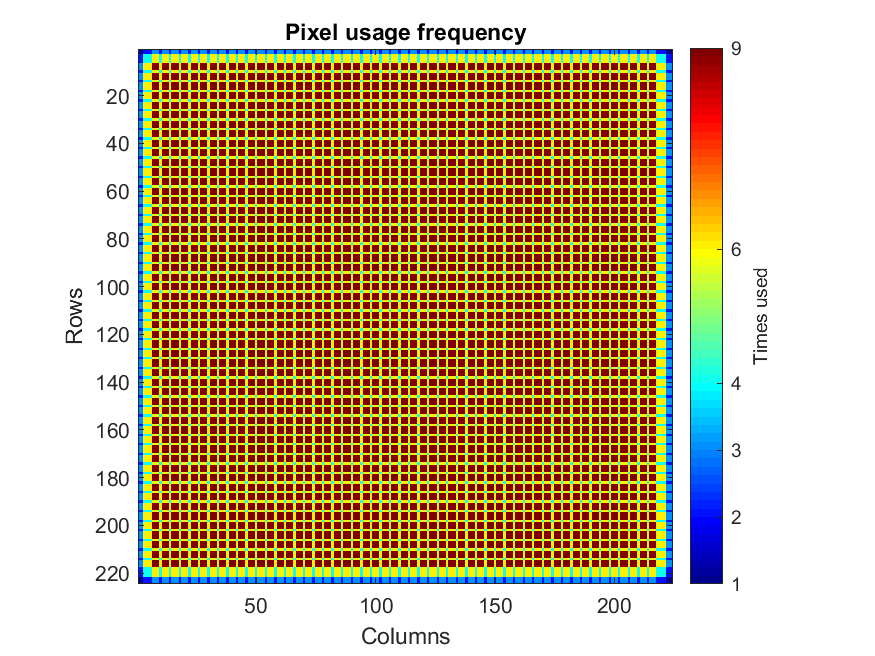
\includegraphics[width=\textwidth]{Images/Scheduling/Conv1-pixel-frequency.png}
	\decoRule
	\caption[Convolutional and Max-Pooling layer input pixel usage frequency using a stride of four]{Convolutional and Max-Pooling layer input pixel usage frequency using a stride of four: Blue inputs are rarely used, while red ones are used frequently.}
	\label{fig:Conv1-pixel-frequency}
\end{figure}

On the other hand, fully-connected layers do not require a specific order for their inputs. However, they need to store partial results for their outputs. Whenever an input is given to the fully-connected layer, it adds it to the partial result of each output after multiplying it with its corresponding weight per output. This creates higher memory requirements for the implementation of the fully-connected accelerator.

Unfortunately, due to the layer-pipelining's significantly increased complexity, this work does not implement it on its accelerators, and it is only presented for completeness and ideas for future work.

\subsubsection{Multi-Inference Strategy}
When multiple accelerators per layer type can be placed into the FPGA device's PL part, they can be utilized simultaneously by running multiple inferences in parallel. The multi-inference strategy schedules two or more images for inference, increasing the platform's overall throughput.

\subsubsection{Image-Pipelining Strategy}
Similar to the multi-inference strategy, when there are multiple accelerators per layer type, multiple images can be fed into the network in a pipelined manner. Every accelerator instance represents a single layer of the network. Hence, the first image can be fed into the first layer. Afterward, when the first layer has generated its outputs, they are fed to the second layer, and the first layer is fed with the second image. This continues for all images to be inferenced. Therefore, when the pipeline is full, all accelerators process different input images from each other. This strategy can decrease the platform's inference latency, and, potentially, the platform's throughput.

\subsection{Amdahl's Law}
\label{sec:Amdahls-Law}
Amdahl's law \cite{Improvements-in-Multiprocessor-System-Design} is a formula that calculates the theoretical speedup in latency of the execution of a fixed workload task, when the system's resources are improved or increased. While speedup was firstly used on parallel processing, it can also be used after any resource enhancement.

Latency is the time required for a system to compute a single task and is defines as:
\begin{equation}
	\label{eqn:latency}
	\begin{split}
		Latency = \frac{1}{v} = \frac{T}{W},\\
		\mbox{v: the task's execution speed},\\
		\mbox{T: the task's execution time},\\
		\mbox{W: the task's execution workload}\\
	\end{split}
\end{equation}

Throughput is the maximum processing rate of a specific task and is defined as:
\begin{equation}
	\label{eqn:throughput}
	\begin{split}
		Throughput = r * v * A = \frac{r * A * W}{T} = \frac{r * A}{L},\\
		\mbox{r: the execution density},\\
		\mbox{A: the execution capacity}\\
	\end{split}
\end{equation}

The speedup is defined for both latency and throughput, as shown in the equations below:
\begin{equation}
	\label{eqn:latency-speedup}
	\begin{split}
		S_{Latency} = \frac{L_1}{L_2} = \frac{T_1 * W_2}{T_2 * W_1} = \frac{1}{(1 - p) + \frac{p}{s}},\\
		\mbox{p: the task's portion that benefits from the resource enhancements},\\
		\mbox{s: the speedup of the task's portion that benefits from the resource enhancements}\\
	\end{split}
\end{equation}
\begin{equation}
	\label{eqn:throughput-speedup}
	S_{Throughput} = \frac{Throughput_2}{Throughput_1}\\
\end{equation}

The maximum theoretical speedup can also be defined as:
\begin{equation}
	\label{eqn:max-speedup}
	MaxSpeedup = \lim_{s \to \infinity} S_{Latency} = \frac{1}{1 - p}\\
\end{equation}

\subsection{AlexNet Characteristics}
\begin{table}[H]
	\caption{Scale and bit-width of input and activations}
	\label{tab:scale-and-bit-width-of-input-and-activations}
	\centering
	\begin{tabular}{llll}
		\toprule
		\textbf{Layer} & \textbf{Scale} & \textbf{Theoretical bit-width} & \textbf{Practical bit-width}\\
		\midrule
			Input & 7 & 8 & 8\\
			Conv1 & 5 & $16 + \lceil \log_2 3 * 11 * 11 \rceil = 25 $ & 17\\
			Conv2 & 5 & $16 + \lceil \log_2 64 * 5 * 5 \rceil = 27$ & 14\\
			Conv3 & 5 & $16 + \lceil \log_2 192 * 3 * 3 \rceil = 27$ & 15\\
			Conv4 & 6 & $16 + \lceil \log_2 384 * 3 * 3 \rceil = 28$ & 15\\
			Conv5 & 5 & $16 + \lceil \log_2 256 * 3 * 3 \rceil = 28$ & 17\\
			FC1 & 5 & $16 + \lceil \log_2 9216 \rceil = 30$ & 17\\
			FC2 & 6 & $16 + \lceil \log_2 4096 \rceil = 28$ & 17\\
			FC3 & 6 & $16 + \lceil \log_2 4096 \rceil = 28$ & 17\\
		\bottomrule\\
	\end{tabular}
\end{table}
